\chapter{Resultados experimentales}
\label{resultados}
\section{Comparación de parámetros $P$ y $N$}
Como se explicó en el \autoref{heurístico}, el algoritmo desarrollado depende de dos parámetros: $G$, la frecuencia con la que realizamos la fase constructiva; y $N$, el número máximo de elementos que puede contener la cola de vuelos extras.\\
Tras realizar varias pruebas, hemos podido comprobar que, como era de esperar, los mejores resultados se obtienen con un parámetro $N$ pequeño y $G$ grande:
\begin{itemize}
	\item Un \textbf{\textit{N} pequeño} implica realizar la fase constructiva con mucha frecuencia. Esto hace que cada pocas iteraciones busquemos un intento de mejora, y por tanto en caso de no conseguir mejorar la solución actual descartaremos la cola de vuelos extras con mucha rapidez.\\
	Un $N$ pequeño también aporta más desviación a los resultados, ya que al descartar colas con mucha facilidad, hace que el problema se reinicie con más frecuencia, y por tanto tenga más aleatoriedad. 
	
	\item Un \textbf{\textit{G} grande} implica que se de más peso a las buenas soluciones que se localizaron en la cola anterior. Por tanto al tener una cola de vuelos extras de gran tamaño, permite que las buenas soluciones tengan una probabilidad mucho mayor que salir antes en el proceso aleatorio de selección de orden de los vuelos para intentar ser colocados.
\end{itemize} 

Los resultados completos de las pruebas realizadas pueden consultarse en el \autoref{anexo1}.

\section{Resultado obtenidos}
Utilizando la configuración de parámetros que hemos obtenido como la más óptima, $N$ pequeño y $G$ grande, resumimos las características principales del problema que hemos obtenido (para ver con detalle los resultados obtenidos consultar el \autoref{anexo1}):

\subsection{Valor de la función objetivo}
Aunque el resultado de la simulación depende de varios parámetros como el problema sobre el que se aplica o el número de vuelos en el problema, todos los problemas tienen características comunes:
\subsubsection{Alto porcentaje de vuelos con solución}
..............................................
\subsubsection{Gran aleatoriedad}
Como ya comentamos, con la configuración de parámetros $G$ y $N$ elegida, obtenemos un grado de aleatoriedad elevado................................

\subsubsection{Evolución de la función objetivo}
En la \autoref{fig: Evolucion función objetivo} se muestra la evolución del valor de la función objetivo en un ejemplo de 100 vuelos con parámetro $N=5$: 
\begin{figure}[H]
	\begin{center}
		\centering
		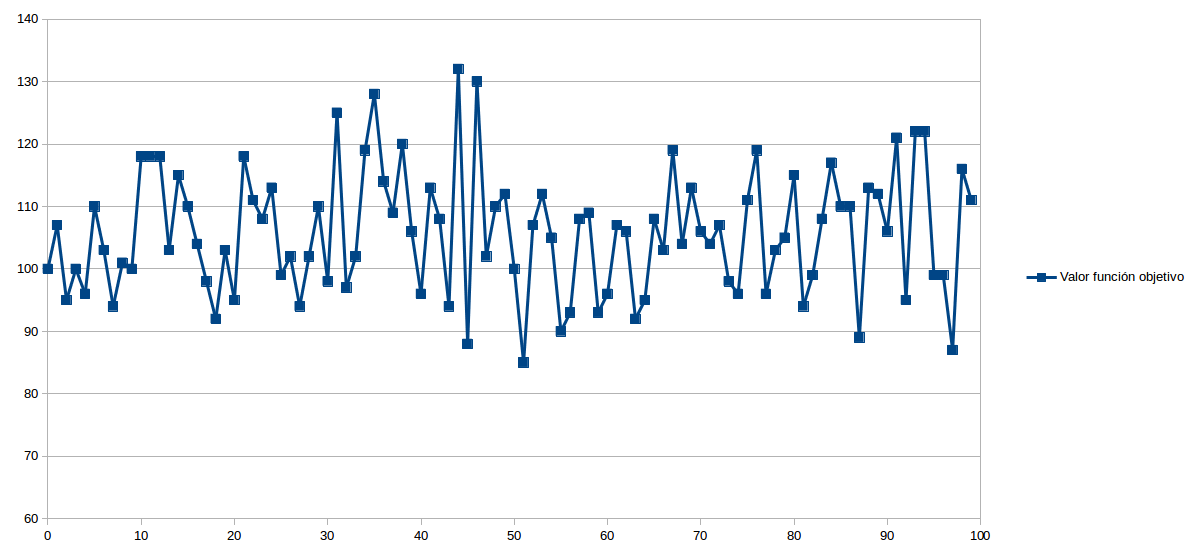
\includegraphics[width=1\textwidth]{./imagenes/resultados/evolucionFuncionObjetivo.png}
		\caption{Evolución función objetivo con $N=5$ y $G=20$ con ejemplo de 100 vuelos}
		\label{fig: Evolucion función objetivo}
	\end{center}
\end{figure}
Como se puede comprobar, en las iteraciones en las que se produce la fase de evaluación y se decide si se descarta la cola, se pueden dar importantes cambios. Por ejemplo, en la \autoref{fig: Evolucion función objetivo} se puede observar como en la iteración con $x=40$ ha habido un descarte de la cola que se había elegido en la anterior fase de mejora, ya que en la siguiente iteración ha habido una gran mejora.\\
Por el contrario en las iteraciones $x=60$ o $x=80$ se puede observar que no se ha descartado la cola de candidatos, ya que el cambio en la función objetivo ha sido mas leve.

\section{Representación gráfica}
A continuación se muestra la representación gráfica obtenida para un problema con 20 vuelos.
\begin{figure}[H]
	\begin{center}
		\centering
		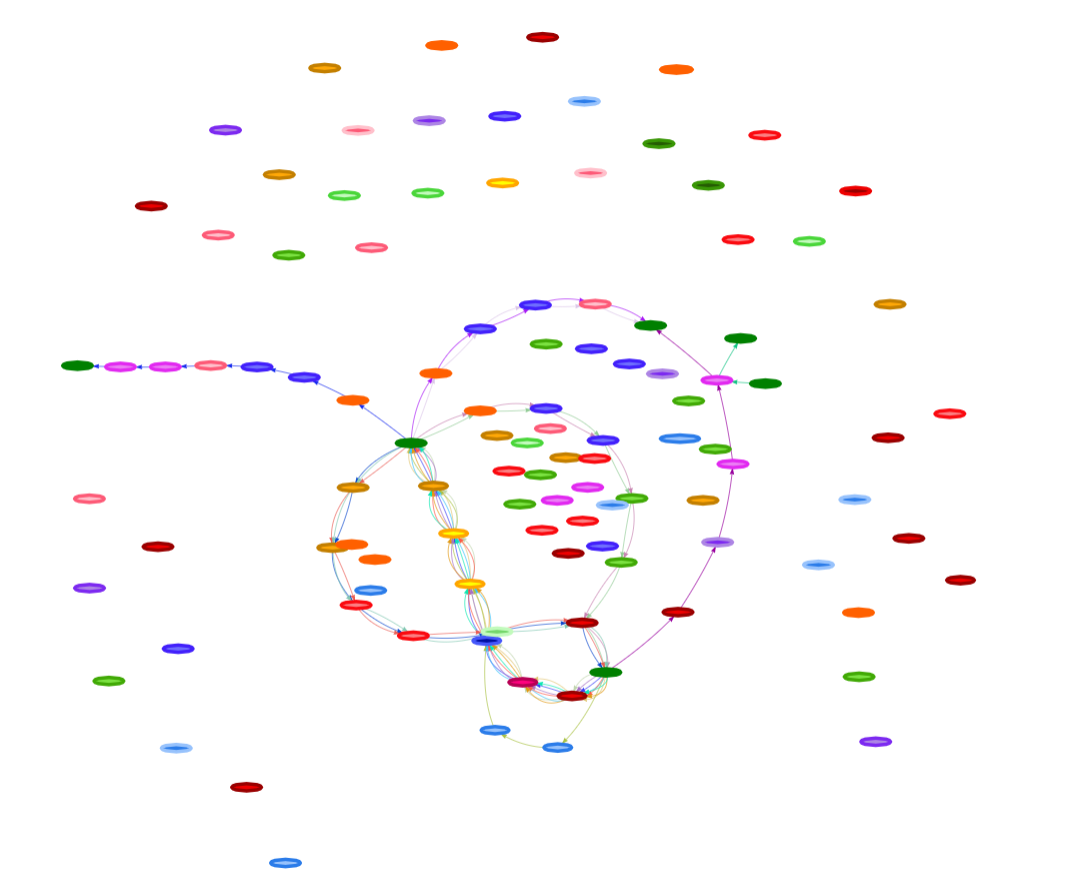
\includegraphics[width=1\textwidth]{./imagenes/resultados/resumenRepresentaion.png}
		\caption{Representación gráfica de un problema de 20 vuelos}
		\label{fig: Representación gráfica de un problema de 20 vuelos}
	\end{center}
\end{figure}

La representación gráfica muestra el resultado final del problema, es decir, se van a representar todos los vuelos a los que se les encontró solución independientemente de los instantes de tiempo en los que estuvieron en tránsito. Por tanto la representación gráfica nos permite observar qué rutas van a ser las más utilizadas.\\
Algunas características de la representación gráfica:
\begin{itemize}
	\item Sólo muestra los vuelos a los que se les encontró solución.
	\item Los waypoints que están ubicados en el mismo sector se marcan del mismo color (si un waypoint pertenece a más de un sector se escoge solamente el primero para simplificar).
	\item Cada vuelo tiene asignado un color para poder identificar su ruta.
	\item En las aristas del grafo representado se indica el instante de tiempo en el que un vuelo realiza ese trayecto
\end{itemize}

\begin{figure}[H]
	\begin{center}
		\centering
		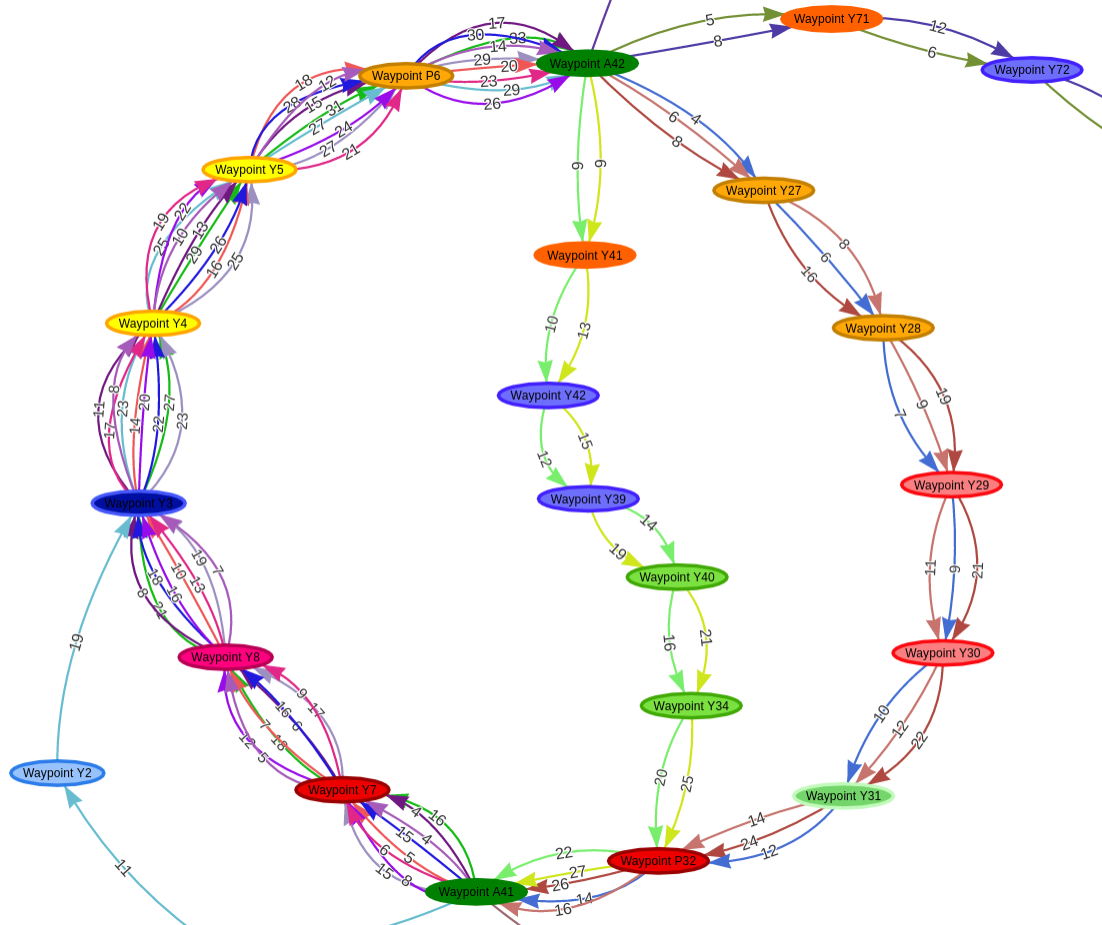
\includegraphics[width=1\textwidth]{./imagenes/resultados/representacionGrafica.png}
		\caption{Ejemplo rutas entre 2 aeropuertos}
		\label{fig: Ejemplo rutas entre 2 aeropuertos}
	\end{center}
\end{figure}

En la \autoref{fig: Ejemplo rutas entre 2 aeropuertos} se puede observar que en el trayecto entre el \textit{Aeropuerto 42} y el \textit{Aeropuerto 41} existen 2 posibles rutas: la rama derecha (más rápida y por tanto con más vuelos) y la rama entral (la ruta alternativa, ya que es más lenta).